\documentclass[a4paper,12pt]{article}
\usepackage[margin=1in]{geometry}
\renewcommand{\tabcolsep}{1 mm}
\usepackage[T2A]{fontenc}			% кодировка
\usepackage[utf8]{inputenc}			% кодировка исходного текста
\usepackage[english,russian]{babel}	% локализация и переносы
\usepackage{graphicx}                % Математика
\usepackage{amsmath,amsfonts,amssymb,amsthm,mathtools} 
\usepackage{mathtext}
\usepackage[T2A]{fontenc}
\usepackage[utf8]{inputenc}

\usepackage{wasysym}

%Заговолок
\author{Бичина Марина 
группа Б04-005 1 курса ФЭФМ}
\title{Отчет по лабораторной работе №2.3.1


Получение и измерение вакуума}
\date{7.04.2021}


\begin{document} % начало документа

\maketitle
\newpage

\section{Аннотация}

\paragraph{Цель работы:} 
\begin{enumerate}
\itemsep0em
\item Измерить объемы форвакуумной и высоковакуумной частей установки
\item Определить скорости откачки системы в стационарном режиме, а также по ухудшению и по улучшению вакуума
\end{enumerate}
\paragraph{Оборудование:}
\begin{enumerate}
\itemsep0em
\item вакуумная установка Б
\end{enumerate}
\section{Теоретическая часть}
\paragraph{}
Вакуумом называется состояние газа, при котором характерная длина свободного пробега молекул в газе $\lambda$ сравнима по порядку величины с характерным линейным размером сосуда $d$, в котором газ находится. Для воздуха при нормальных условиях $\lambda \sim 10^{-5}$.

Техническим вакуумом называют состояние газа при котором его давление меньше атмосферного (P<$P_{\text{атм}}$).

Различают 3 вида технического вакуума:
\begin{enumerate}
\itemsep0em
\item Низкий, когда средняя длина свободного пробега молекул газа значительно меньше характерного линейного размера объема, то есть $\lambda < d$
\item средний $\lambda \sim d$
\item высокий (глубокий) $\lambda > d$. Газ в этом состоянии называется ультраразреженным 
\end{enumerate}
\paragraph{}
Также для характеристики степень разреженности газового 
потока вакуумных систем можно использовать число Кнудсена
	
	\begin{equation}
		Kn = \frac{\lambda}{d}, 
	\end{equation}

	$\lambda$ -- длина свободного пробега молекул газа, $d$ -- характерный размер системы. \\
	
	Тогда в зависимости от значений числа Кнудсена можно выразить:
\begin{enumerate}
\itemsep0em
\item низкий вакуум -- $Kn \ll 1$
\item средний вакуум -- $Kn \sim 1$
\item высокий вакуум -- $Kn \gg 1$
\end{enumerate}	
\paragraph{}
Выпишем основные формулы, отображающие теоретические зависимости между исследуемыми величинами, необходимые в данной работе. Здесь и далее $L$ -- единица измерения длины, $M$ -- массы, $T$ --  времени в системе LMT
\begin{enumerate}
\itemsep0em
\item Быстрота откачивающего действия (скорость откачки) вакуумной системы $S [L^3T^{-1}]$ -- объем газа, проходящий через рассматриваемое сечение вакуумпровода в единицу времени при текущем давлении в данном сечении:
\[S = \dfrac{dV}{dT}\]
Следовательно быстродействие насоса $S_{\text{н}}$ определяется как:
\begin{equation}
 S_{ \text{н} } = \dfrac{dV_{ \text{н} }}{dt}
\end{equation}
А эффективная скорость откачки камеры $S_0$:
\begin{equation}
S_0 = \dfrac{ dV_0 }{ dt } 
\end{equation}
\item Падение давления вдоль вакуумпровода $ \Delta P = P_1 - P_2 $. Oпределяется его пропускной способностью (проводимостью) $ U [L^3 T^{-1} ] $:
\[ U = \dfrac{Q}{P_1 - P_2} \]
где $Q [L^2 M T^{-3}]$ - поток газа через вакуумпровод с соответствующими давлениями на концах.
\item Величина $Z [L^{-3}T]$, обратная проводимости, называется импедансом вакуумпровода:
\[Z=\dfrac{1}{U}\]
В общем случае указанные величины $S$, $U$, $Q$, $Z$ как и сами давления $P_1$ и $P_2$ зависят от времени. Но в конце процесса откачки устанавливается квазистационарный режим, при котором поток газа становится практически постоянным и равным количеству поступающего в систему газа в единицу времени вследствие наличия течей, т.е. нарушения герметичности (в основном в местах механического соединения отдельных узлов вакуумной системы). Для стационарного режима можно записать условие непрерывности потока откачиваемого газа:
\[P_1 S_0 = PS = P_2 S_{\text{н}} = Q \]
\item Получим основное уравнение вакуумной техники
\begin{equation}
\dfrac{1}{S_0} = \dfrac{1}{S_{ \text{н} }} + \dfrac{1}{U}
\end{equation}
\item Проводимость длинного трубопровода
\[U_{\text{тр}} = \dfrac{Q}{P_2 - P_1} = P\dfrac{\pi R^4}{8 \nu L} \sim \dfrac{R^4}{L} \dfrac{P}{\sqrt{Tm}}\]
\[U_{\text{тр}} = \dfrac{Q}{P_2 - P_1} = \dfrac{4}{3} \dfrac{R^3}{L}\sqrt{\dfrac{2 \pi k T}{m}} \sim \dfrac{R^3}{L} \sqrt{\dfrac{T}{m}} \]
В случае последовательного соединения:
\[U_{\Sigma} = \dfrac{1}{Z_{\Sigma}} = \dfrac{1}{\Sigma Z_i}\]

\[S_0 = \dfrac{S_{\text{н}}U_{\Sigma}}{S_{\text{н}} + U_{\Sigma}} = \dfrac{S_{\text{н}}}{\dfrac{S_{\text{н}}}{U_{\Sigma}} + 1} \approx S_{\text{н}} \]	
\item Уравнение откачки газа
\begin{equation}
P(t) = P_1 \exp \left( -\dfrac{S_0}{V_0} t \right)
\end{equation}
\end{enumerate}
\subsection{Описание экспериментальной установки}

\begin{figure}[h]
	\centering
	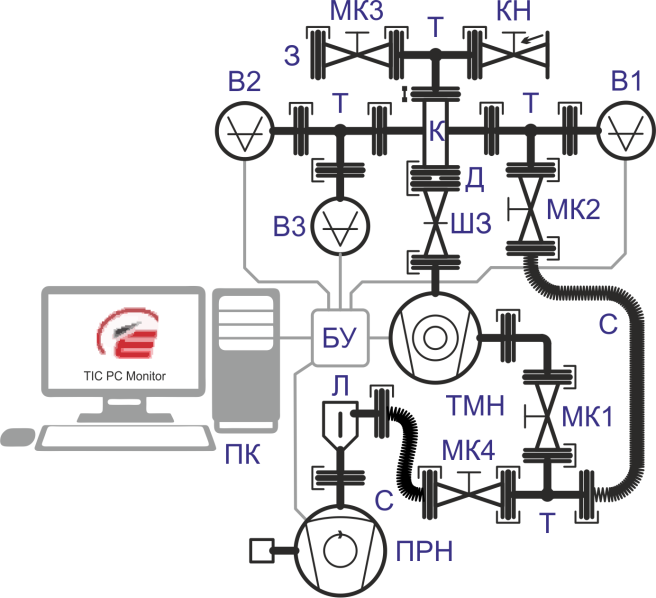
\includegraphics[width=0.5\linewidth]{fig.png}
	\caption{Схема экспериментальной установки}
	\label{setup1}
\end{figure}

\begin{figure}[h]
\begin{center}
\begin{minipage}[h]{0.45\linewidth}
	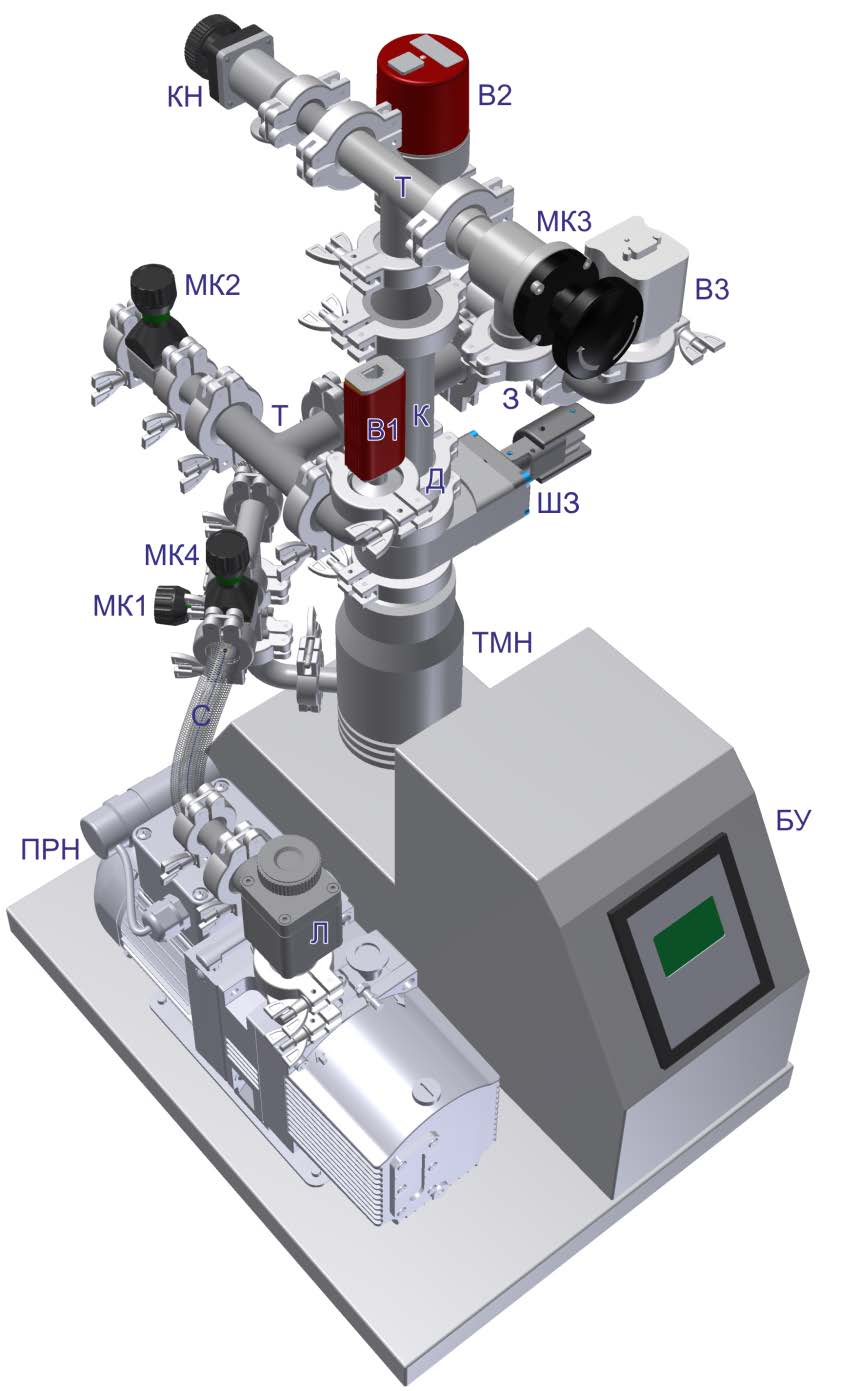
\includegraphics[width=0.9\linewidth]{fig1.jpg}
	\caption{Внешний вид экспериментальной установки (спереди)} 
	\label{front}
\end{minipage}
\hfill
\begin{minipage}[h]{0.45\linewidth}
	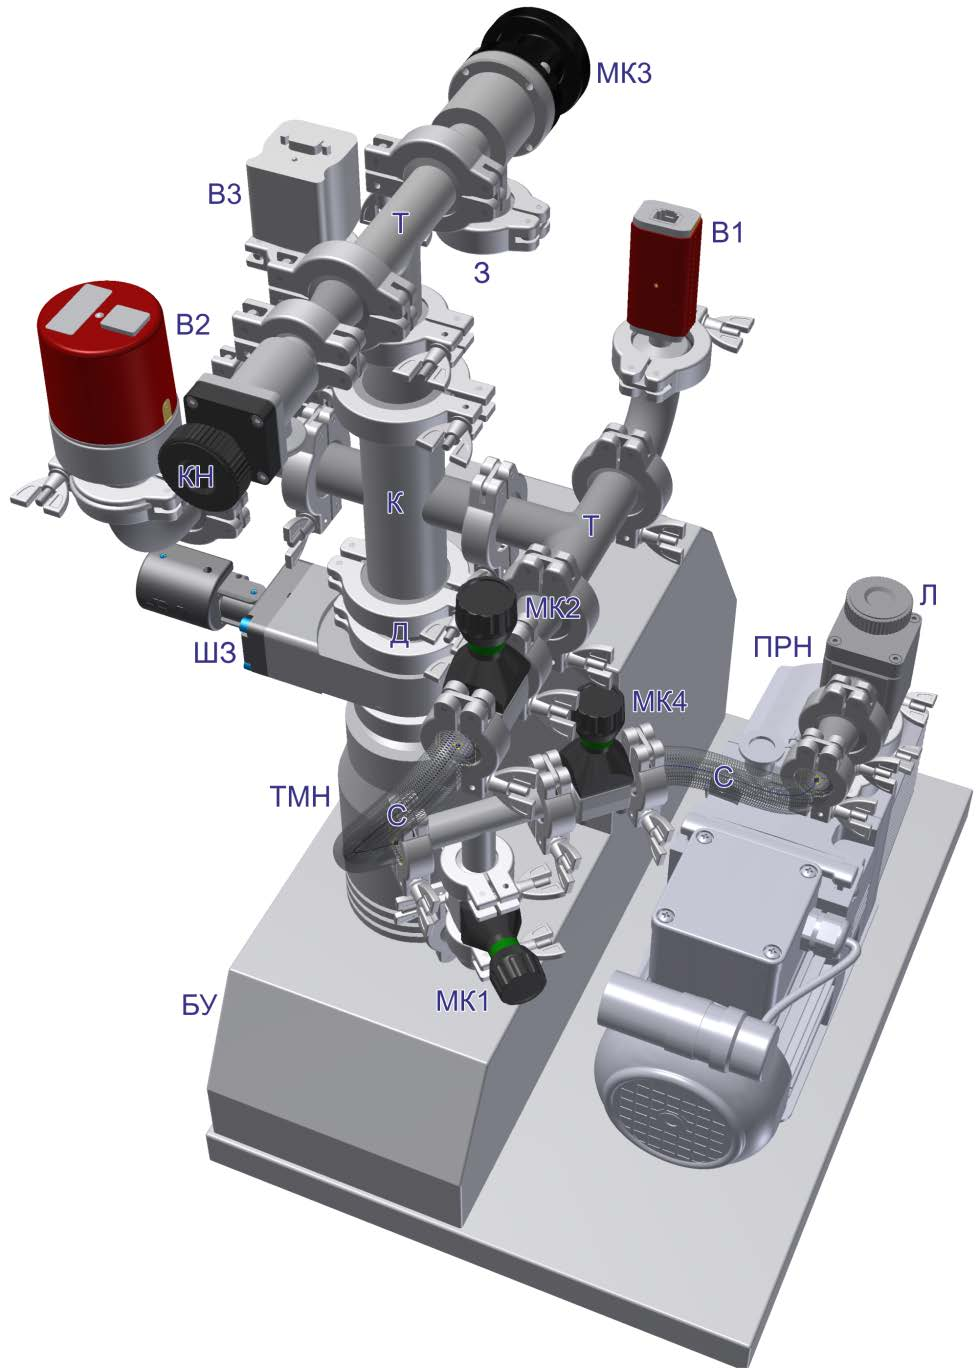
\includegraphics[width=1\linewidth]{fig2.jpg}
	\label{back}
	\caption{Внешний вид экспериментальной установки (сзади)}
\end{minipage}
\end{center}
\end{figure}

\noindent \textbf{Обозначения на рисунках 1, 2, 3:}\\
БУ -- Блок управления \\
ПРН -- пластинчато-роторный насос  \\
ТМН -- турбомолекулярный насос \\
К -- Вакуумная камера \\
ШЗ -- Шиберный затвор \\
МК1-4 -- Мембранные краны \\
В1 -- Терморезисторный вакууметр \\
В2 -- Магнитронный вакууметр \\
В3 -- Термоэлектронный вакууметр \\
КН -- Кран-натекатель \\
Л -- Маслоуловитель \\
З -- Заглушка \\
Д -- Диафрагма \\
С -- Сильфоны \\
Т -- Тройники \\
ПК -- Компьютер \\

\section{Ход работы}

\begin{enumerate}
\renewcommand{\labelenumii}{\arabic{enumii}.}

\item \textbf{Подготовка к работе и подключение системы управления }
\begin{enumerate}
	\item
	Сопоставим элементы схемы (рис. \ref{setup1}) с соответсвующими частями самой установки.
	\item
	Последовательно откроем краны МК1, МК2, МК3, МК4 поворотом ручек против часовой стрелки (зелёные метки на кранах должны быть максимально видны), потом откроем шибер ШЗ (ручка шибера в крайнем дальнем от установки положении). 
	\item
	\textit{Впустим атмосферный воздух в установку через кран-натекатель КН}. Ручку тонкой регулировки КН со шкалой плавно вращаем до упора против часовой стрелки (около 14-ти полных оборотов). 
	\item
	\textit{Подготовим систему к форвакуумной откачке.} Закроем КН плавно вращая ручку тонкой регулировки со шкалой до упора  по часовой  стрелке  (около  14-ти  полных  оборотов).  Закроем кран МК3, шибер ШЗ, а Краны МК1, МК2, МК4 оставим открытыми. Определим по схеме, по каким магистралям и какие объёмы будут откачиваться форвакуумным насосом при данном состоянии кранов. 
	\item \textit{Включим питание экспериментального стенда и ПК.} 
	\item \textit{Запустим программу управления TIC PC Monitor.}
	\item \textit{Установим связь между БУ, насосами и вакууметрами.}
	\item \textit{Выберем данные для записи в файл.}
	\item \textit{Включим запись данных в файл.}
\end{enumerate}

\item \textbf{Определение откачиваемого объёма и измерение скорости откачки форвакуумным насосом.}
\begin{enumerate}
	\item \textit{Откачаем установку форвакуумным насосом ПРН.} Отметим время запуска  в тетради. Откачаем установку до предельного давления, которое можно определить под динамике показателей вакууметров.
	\item \textit{Присоединим к установке сильфон с воздухом при атмосферном давлении.} Отсоединим заглушку З от крана МК3 (\textbf{кран МК3 закрыт!}). Протрём вакуумные поверхности сильфона С, заглушки З, а также уплотнительные кольца безворсовой тканью смоченной обезжиривающей жидкостью. Установите заглушку З на один конец гибкого сильфона, а другой конец присоедините к крану МК3. \\ При этом в сильфоне между заглушкой и краном будет <<заперто>> 252 мл воздуха при атмосферном давлении. 
	\item \textit{Выровняем давления в сильфоне С и вакуумной камере К экспериментального стенда.} Перекроем откачку вакуумной камеры К, закрыв кран МК2. Далее \textbf{предельно  плавно},  не допуская  резкого  изменения  показаний  вакуумметра В1, откроем кран МК3 для распространения <<запертого>> воздуха по объёму вакуумной камеры К (насос ПРН должен оставаться \textbf{включённым!}). Зафиксируем установившиеся показания  вакуумметра В1. Сделаем  выводы  о точности  его  показаний  в данном  диапазоне  измерений. 
	\item \textit{Выровняем давление вакуумной камеры К и форвакуумной магистрали установки.} Закроем  краны МК1  и МК4.  Далее  плавно  откроем  кран  МК2. Зафиксируем установившиеся показания вакууметра В1. Насос ПРН при этом остаётся \textbf{включенным} и откачивает только масляную ловушку и сильфон С до крана МК4. 
	\item \textit{Выровняйте  давление  во  всей  установке,  включая  объем  турбомолекулярного насоса ТМН.} Плавно откроем кран МК1, запустив воздух в объём насоса ТМН. Зафиксируем установившиеся значения вакууметра В1 (насос ПРН должен оставаться \textbf{включённым!}). 
	\item \textit{Напустим в установку воздух до атмосферного давления.} Выключим насос ПРН и откроем кран МК4. Ручку тонкой регулировки КН со шкалой плавно вращаем до упора против часовой стрелки.
	\item \textit{Подготовьте  установку  к  повторному  выполнению  части II  задания.}
	Закроем КН плавно вращая ручку тонкой регулировки со шкалой до упора  по часовой  стрелке  (около  14-ти  полных  оборотов).  Закроем кран МК3.
	\item Измерения по пп. 1-7 повторим ещё 1-2 раза, каждый  раз фиксируя время начала работы форвакуумного насоса ПРН. Если  достигается  приемлемая  повторяемость,  можно  переходить к следующей части задания.
	
	\emph{Определим объёмы вакуумных частей установки согласно пп 1. Определим скорость откачки системы насосом ПРН по улучшению вакуума во время откачки согласно пп. 2.}
	
\end{enumerate}

\item \textbf{Измерение скорости откачки турбомолекулярным насосом и определение предельного вакуума}
\begin{enumerate}
	\item \textit{Отсоединим сильфон от установки.} Отсоединим сильфон он установки и установим заглушку З на кран МК3. Откроем кран МК3, чтобы убрать из установки запертый объём воздуха между заглушкой З и краном МК3.
	\item \textit{Откачаем установку форвакуумным насосом ПРН.}
	\item \textit{Откачаем объём турбомолекулярным насосом ТМН.} Откроем  шибер ШЗ,  закроем  кран МК2.  Определим  по схеме, по каким магистралям и какие объёмы будут откачиваться двумя насосами при данном состоянии кранов. Отметим время начала работы насоса ТМН. Откачайте  установку  до  предельного  давления,  которое  можно по динамике показаний вакууметров В2 и В3. \\
	Проанализируем работу вакууметров убедимся,что терморезисторный  вакуумметр В1  достиг  своего  предела  измерений, в то время как инверсно-магнетронный вакуумметр В2 включился и отображает  корректное  давление  в системе.  Зафиксируем  предельное  давление в высоковакуумной части установки и время откачки установки насосом ТМН. 
	\item \textit{Проведём обезгаживание наклалённой спирали включившегося термоэлектронного вакууметра В3 для устранения искажений его показаний.} После дегазации сравним показания вакууметров В2 и В3.
	\item \textit{Определите уровень течей и скорость откачки системы.} Закроем  шибер  ШЗ,  при  этом  давление  в  системе  начнёт  повышаться за счёт наличия течей. Получим таким образом зависимость показаний вакууметров В2 и В3 от времени. Когда давление превысит $10^{-3}$ мбар, снова откроем шибер. \\ 
	Получим зависимость показаний В2 и В3 от времени после открытия шибера. Снова зафиксируем предельное давление. Время снятия показаний по пп. 5 не должно превышать 10 мин.
	\item Измерения  по пп. 5  повторим  ещё 1-2  раза,  каждый  раз  фиксируя время закрытия и открытия шибера ШЗ. Если  достигается  приемлемая  повторяемость,  перейдём к следующей части задания.  
\end{enumerate}


\end{enumerate}
\end{document}